\begin{figure*}
\begin{center}
  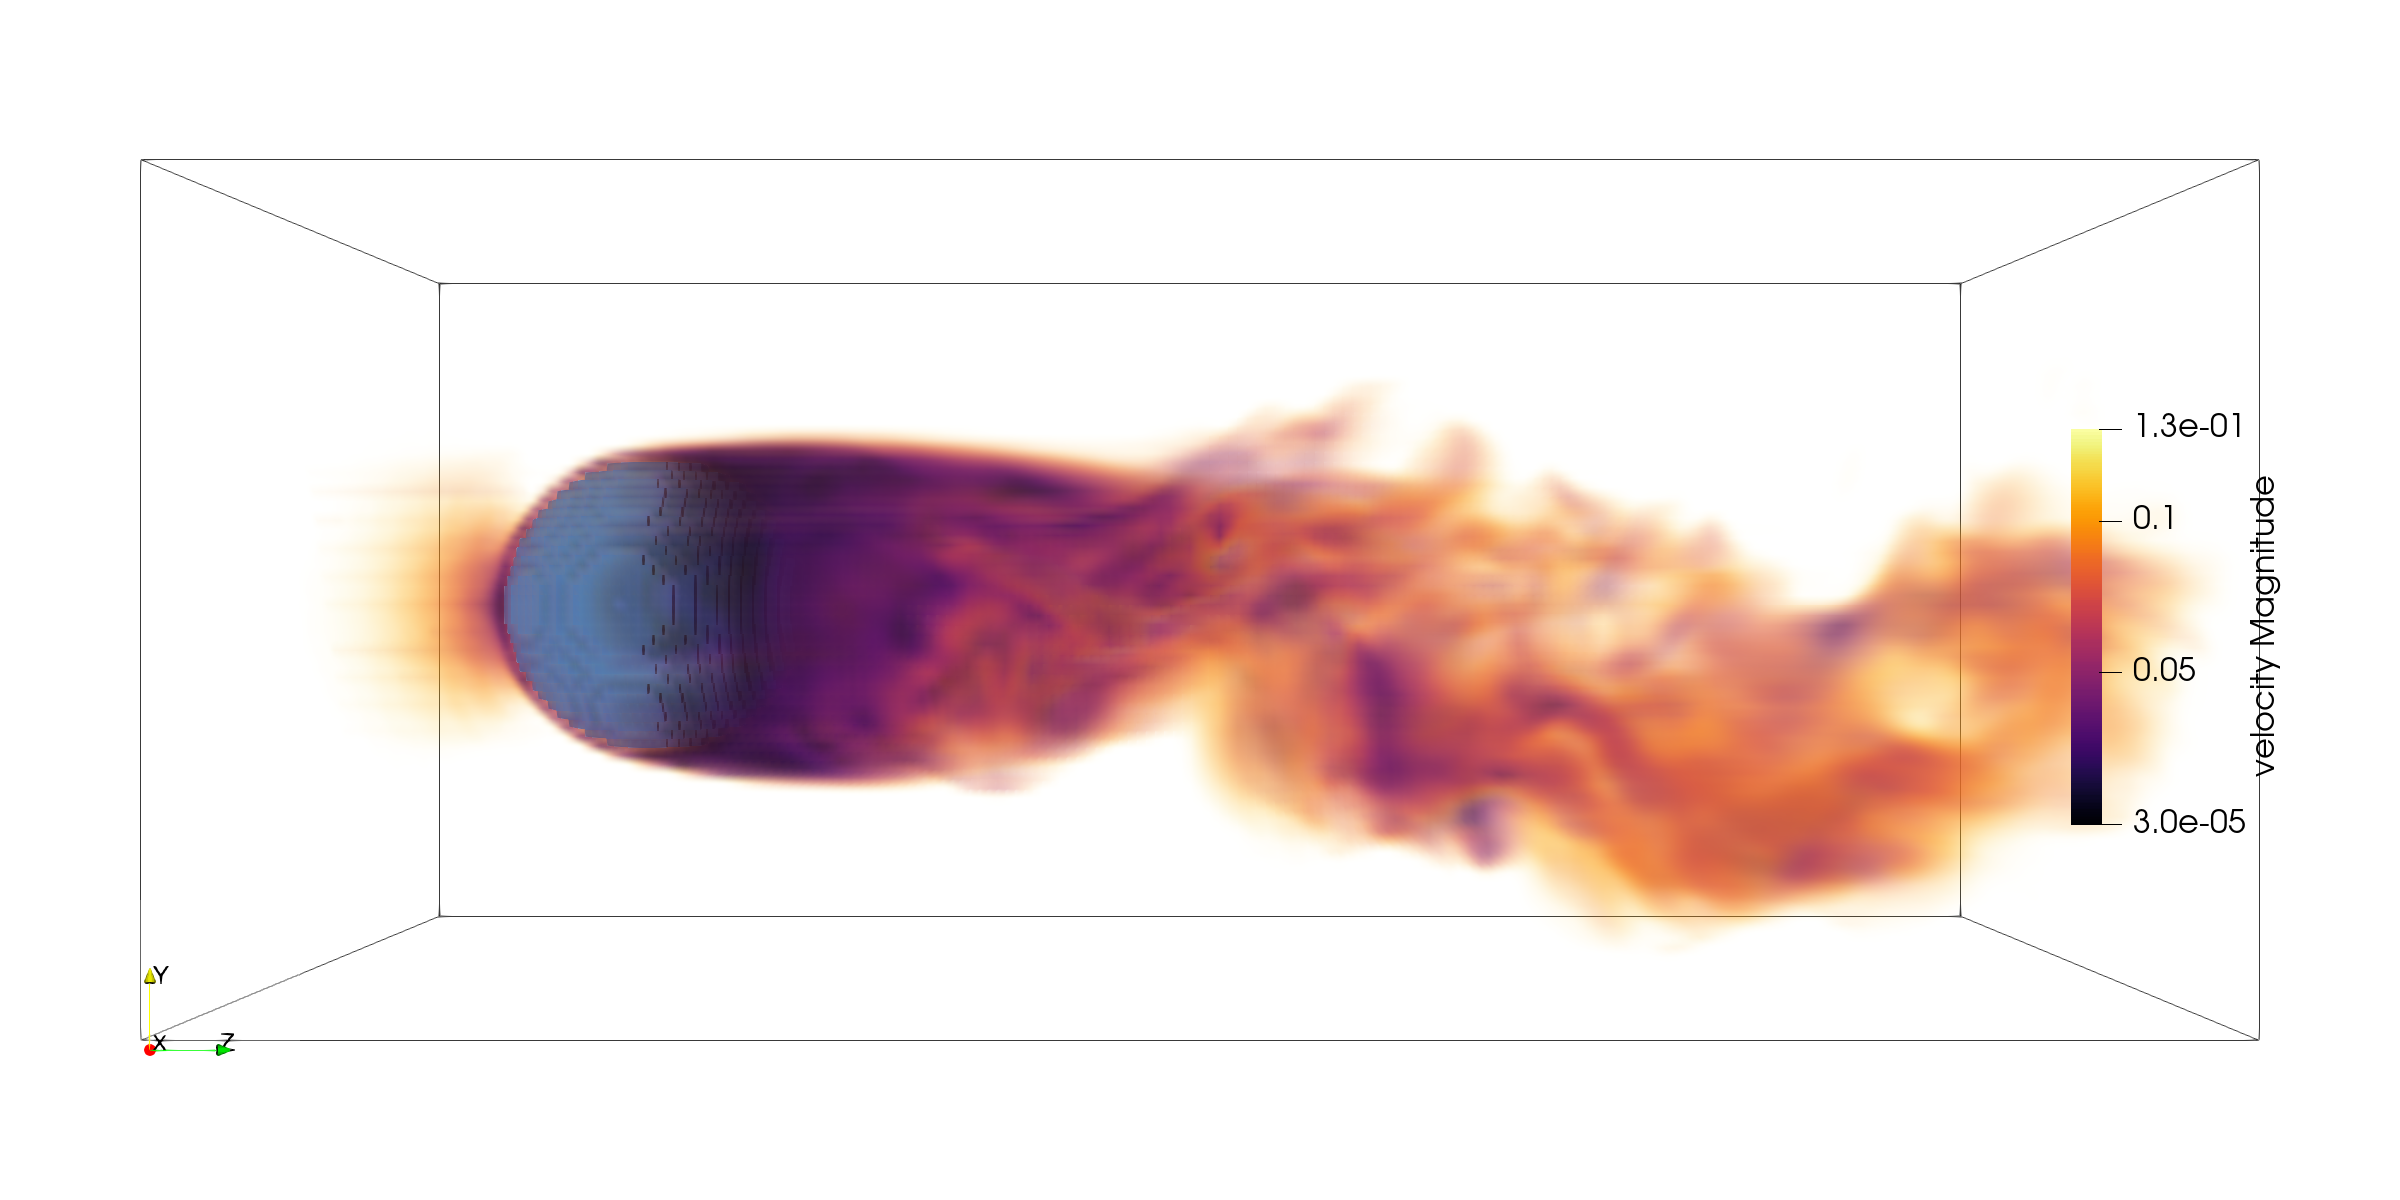
\includegraphics[width=\linewidth]{purple_render_01.png}
\end{center}
\caption{This is a frame from one of our demo movies,
  where we model fluid flowing around a sphere.
  This is a volumetric render of velocity magnitude. 
  We see turbulence emerge, as this setup has a high Reynold
  s number..
  The simulation domain was a $79 \times 79 \times 190$ 
  $D3Q27$ lattice. 
  This film ran the simulation for $20,000$ iterations,
  creating a frame every $10$ iterations.
It took $\approx 49$ minutes to run, 
and generated $\approx 300$Gb of data.
Paraview took almost $9$ hours to render the film.}
\label{fig:movie-frame}
\end{figure*}

\section{Intoduction}

The lattice Boltzmann method (LBM) 
is a framework for numerically modelling fluid dynamics
that maps well to GPU compute.
However LBM based models have traditionally struggled to 
resolve turbulent flows.
Given that the visual interest of fluid dynamics is often 
derived from turbulence, this has limited the use of LBM 
for graphics applications.

Active research has rapidly evolved LBM based models,
and new collision operators like CM-MRT (see section \ref{sec:cm-mrt})
have greatly improved accuracy when modelling turbulent flows.
CM-MRT has seen adoption by graphics 
researchers \cite{Li2020, Li2024, Lyu2021} due
to its ability to better resolve visually interesting
fluid dynamics.

The proposal for my final project was to
implement a GPU based LBM simulation utilizing the CM-MRT collision 
operator.
I was able to implement most of the ideas from
my proposal, using CM-MRT operator in particular.
My implementation is described and discussed in section 
\ref{sec:implementation}.
In section \ref{sec:related_work} I explore the theory
of what I implemented as well as related work.
Future work is discussed in section \ref{sec:futurework}.


My project fell short of my proposal in a few places.
I had planned on implementing a more advanced fluid-solid
interaction, as described in \cite{Lyu2021}.
In the end I only supported a simple bounce-back operator 
(see section \ref{sec:ic-and-bc}) and only implemented a mechanism
for adding spheres rather than arbitrary shapes.
There was also an adaptive relaxation rate scheme from \cite{Li2020}
that would be have been much closer to the state-of-the-art for 
collision operators.
Lastly, I didn't implement the tracer particle based rendering
I had originally proposed and relied entirely on Paraview 
for all my post-processing.

My goals for the project were to to gain experience 
with both GPU programming and 
LBM based modelling.
I succeeded on both of these counts.
I feel far more confident in my ability to utilize compute shaders,
with the added bonus of learning about computer algebra based
code generation.
My greatest success though is on the theory side.
I have gained a foothold into
the state of the art for LBM based methods and
the research being conducted in this area.
